\subsection{Tấn công Brute Force}
\subsubsection{Tấn công Brute Force là gì?}
Tấn công Brute Force là một loại tấn công mạng, trong đó bạn có một phần mềm, xoay vòng các ký tự khác nhau, kết hợp để tạo ra một mật khẩu đúng. Phần mềm Brute Force Attack Password Cracker đơn giản sẽ sử dụng tất cả các kết hợp có thể để tìm ra mật khẩu cho máy tính hoặc máy chủ mạng. Nó rất đơn giản và không sử dụng bất kỳ kỹ thuật thông minh nào. Vì phương pháp này chủ yếu dựa trên toán học, phải mất ít thời gian hơn để crack mật khẩu, bằng cách sử dụng các ứng dụng Brute Force thay vì tìm ra chúng theo cách thủ công. Nói phương pháp này dựa trên toán học vì máy tính làm rất tốt các phép toán và thực hiện chúng trong vài giây, nhanh hơn rất nhiều lần so với bộ não con người (mất nhiều thời gian hơn để tạo ra các sự kết hợp). Tấn công Brute Force là tốt hay xấu tùy thuộc vào người sử dụng nó. Nó có thể được bọn tội phạm mạng cố gắng sử dụng để hack vào một máy chủ mạng, hoặc nó có thể được một quản trị viên mạng dùng để xem mạng của mình được bảo mật có tốt không. Một số người dùng máy tính cũng sử dụng các ứng dụng Brute Force để khôi phục mật khẩu đã quên \cite{hofstede2017flow}.

\subsubsection{ Mục đích của tấn công Brute Force}

\begin{itemize}
    



\item \textbf{Đánh cắp dữ liệu cá nhân}:

Xâm nhập vào các tài khoản cá nhân của người dùng có thể cung cấp một kho báu dữ liệu, từ chi tiết tài chính và tài khoản ngân hàng đến thông tin y tế bí mật. Truy cập vào một tài khoản cho phép kẻ tấn công giả mạo danh tính của một người, đánh cắp tiền của họ, bán thông tin đăng nhập của họ cho bên thứ ba, hoặc sử dụng thông tin để tiến hành các cuộc tấn công lớn hơn.

Dữ liệu cá nhân và thông tin đăng nhập cũng có thể bị đánh cắp thông qua các vụ vi phạm dữ liệu doanh nghiệp mà các kẻ tấn công có thể truy cập vào cơ sở dữ liệu nhạy cảm của tổ chức.

\item \textbf{Lây nhiễm Malware}

Các cuộc tấn công Brute Force thường không phải là cá nhân. Một hacker có thể chỉ muốn tạo ra sự hỗn loạn và trưng bày kỹ năng độc hại của họ. Họ có thể làm điều này bằng cách lây nhiễm Malware qua email hoặc tin nhắn dịch vụ Short Message (SMS), ẩn Malware trong một trang web giả mạo được thiết kế để trông giống như một trang web hợp pháp, hoặc chuyển hướng khách truy cập trang web đến các trang web độc hại.

Bằng cách nhiễm Malware vào máy tính của người dùng, kẻ tấn công sau đó có thể tiến vào các hệ thống và mạng kết nối và tiến hành các cuộc tấn công mạng lớn hơn đối với tổ chức.

\item  \textbf{Chiếm đoạt hệ thống cho hoạt động độc hại}

Các cuộc tấn công Brute Force có thể đóng một vai trò trong việc các hành động độc hại tấn công rộng lớn sử dụng nhiều thiết bị, gọi là một botnet. Điều này thường là một cuộc tấn công từ chối dịch vụ phân tán (DDoS) nhằm mục tiêu làm cho các phòng thủ bảo mật và hệ thống của mục tiêu trở nên yếu đuối.

\item \textbf{Phá hủy uy tín của một công ty hoặc trang web}

Các cuộc tấn công Brute Force thường được tiến hành với mục tiêu đánh cắp dữ liệu từ một tổ chức, điều này không chỉ gây thiệt hại tài chính mà còn gây ra tổn thương uy tín lớn. Các trang web cũng có thể bị mục tiêu với các cuộc tấn công gây ra việc ô nhiễm với văn bản và hình ảnh khiếm nhã hoặc xúc phạm, từ đó làm suy giảm uy tín của họ, có thể dẫn đến việc họ bị xóa khỏi mạng.

\subsubsection{ Nguyên nhân dẫn đến cuộc tấn công Brute Force}
\end{itemize}
\begin{itemize}
    \item Mật khẩu yếu là một trong những nguyên nhân chính khiến tài khoản trở thành mục tiêu của tấn công Brute Force. Mật khẩu ngắn, sử dụng chỉ các ký tự dễ đoán hoặc không có sự kết hợp của chữ cái, số và ký tự đặc biệt là dễ bị tấn công.
    \item Nếu tài khoản sử dụng một mật khẩu mặc định hoặc dễ đoán, nó có thể trở thành mục tiêu dễ dàng cho các cuộc tấn công Brute Force. Các mật khẩu mặc định thường được biết đến và được kẻ tấn công sử dụng để kiểm tra hàng loạt các tài khoản.
    \item Nếu không có các biện pháp bảo mật phòng thủ, như giới hạn số lần đăng nhập thất bại hoặc sử dụng CAPTCHA, tài khoản có thể trở thành mục tiêu cho các tấn công Brute Force. Việc không có các biện pháp bảo mật này cho phép kẻ tấn công thử hàng nghìn hoặc thậm chí hàng triệu mật khẩu trong một thời gian ngắn mà không gặp phải rào cản \cite{stiawan2019investigating}.
    \item Một tài khoản có thể thu hút sự chú ý của kẻ tấn công vì nó chứa thông tin quan trọng hoặc có quyền truy cập vào các tài nguyên quan trọng. Trong trường hợp này, kẻ tấn công có thể quyết định dành thời gian và tài nguyên để thực hiện tấn công Brute Force.
    \item Một lý do khác là sự lạc quan của người sử dụng về mức độ bảo mật của mật khẩu của họ. Họ có thể sử dụng mật khẩu dễ đoán hoặc sử dụng mật khẩu giống nhau cho nhiều tài khoản khác nhau, không thay đổi mật khảu thường xuyên, làm cho chúng trở thành mục tiêu dễ dàng cho các tấn công Brute Force.
\end{itemize}
\subsubsection{Các loại tấn công Brute Force phổ biến }
\begin{itemize}
    \item Tấn công Simple Brute Force: Sử dụng một cách tiếp cận có hệ thống để “đoán” username hay password, không cần dựa vào external logic.
    \item Tấn công Hybrid Brute Force: Bắt đầu từ external logic để xác định các tổ hợp password có khả năng thành công cao nhất. Sau đó tiếp cận với Simple Brute Force Attack để thử nhiều tổ hợp nhất có thể.
    \item Tấn công Dictionary: Đoán username hoặc password bằng cách sử dụng một từ điển các xâu hay cụm từ khả thi.
    \item Tấn công Rainbow Table: Rainbow Table là một bảng được tính toán trước để so khớp với kết quả của các hàm hash. Nó có thể dùng để đoán một hàm có độ dài xác định và chứa một tập hợp kí tự cụ thể.
    \item Tấn công Reverse Brute Force: Sử dụng một password chung hay một tập hợp các password để thử với nhiều username khả thi. Loại tấn công này nhắm vào một mạng người dùng mà các hacker đã lấy được dữ liệu trước đó.
    \item Tấn công Credential Snuffing: sử dụng các cặp password-username đã biết trước, và thử chúng trên nhiều website khác nhau. Sở dĩ vì có không ít người dùng có thói quen sử dụng cùng một cặp password-username trên nhiều hệ thống khác nhau.

\end{itemize}
\subsubsection{ Các công cụ dùng trong tấn công}
 Việc đoán mật khẩu email hoặc trang web mạng xã hội của người dùng có thể là một quá trình tốn nhiều thời gian, đặc biệt nếu tài khoản có mật khẩu mạnh. Để đơn giản hóa quá trình này, hacker đã phát triển phần mềm và công cụ để giúp họ bẻ khóa mật khẩu.
Các công cụ tấn công brute-force bao gồm các ứng dụng bẻ khóa mật khẩu, bẻ khóa các tổ hợp tên người dùng và mật khẩu mà sẽ rất khó để một người tự bẻ khóa. Các công cụ tấn công brute-force thường được sử dụng bao gồm:
\begin{itemize}
    \item Aircrack-ng:
Một bộ công cụ đánh giá an ninh mạng Wi-Fi để giám sát và xuất dữ liệu và tấn công một tổ chức thông qua các phương pháp như điểm truy cập giả mạo và chèn gói.
\item John the Ripper:
Một công cụ khôi phục mật khẩu mã nguồn mở hỗ trợ hàng trăm loại mật mã và băm, bao gồm mật khẩu người dùng cho macOS, Unix và Windows, máy chủ cơ sở dữ liệu, ứng dụng web, lưu lượng truy cập mạng, khóa cá nhân được mã hóa và tệp tài liệu.
\item Hydra:
Hydra là một nền tảng mở, được cộng đồng bảo mật và những kẻ tấn công liên tục phát triển các mô-đun mới. Nó có thể tấn công hơn 50 giao thức và trên nhiều hệ điều hành khác nhau.
\item L0phtCrack:
Một công cụ bẻ khóa mật khẩu Windows. Nó sử dụng bảng cầu vồng, từ điển và các thuật toán đa xử lý.
\item Burpsuite:
Burpsuite không phải là 1 công cụ chuyên dụng để tấn công brute-force, tuy nhiên bạn hoàn toàn có thể tùy chỉnh đầu vào bộ mật khẩu để hướng tới 1 cuộc tấn công brute-force tùy ý.

\end{itemize}
\subsubsection{ Biện pháp ngăn chặn tấn công Brute Force}
\textbf{Đối với người dùng:}

\begin{itemize}
     \item Không sử dụng thông tin liên quan đến bản thân mà có thể lấy được trên mạng như tên, ngày sinh hay địa chỉ của mình…
    \item Có càng nhiều ký tự càng tốt: việc sử dụng từ 10 ký tự trở lên có thể khiến cho tấn công, lưu trữ tốn rất nhiều thời gian, và tài nguyên, thời gian có thể lên cả năm trời.
   \item Kết hợp các chữ cái, số và các ký hiệu đặc biệt \cite{ayankoya2019brute}.
    \item Tránh sử dụng những mật khẩu đơn giản như: 123456, password,…
     \item Bên cạnh đó việc không sử dụng cùng 1 mật khẩu trên nhiều tài khoản khác nhau có thể tránh tối đa hậu quả khi bị mất mật khẩu,
    \item Nên thay đổi mật khẩu thường xuyên: Đây là cách để thoát khỏi các vụ rò rỉ thông tin khi bị Brute Force Attack tấn công. Bởi nếu không may bạn từng là nạn nhân trong cuộc tấn công trước đó, tin tặc có thể dùng dữ liệu đã đánh cắp để tiếp tục đăng nhập vào tài khoản của người dùng \cite{ayankoya2019brute}.

\end{itemize}



\textbf{Đối với quản trị viên:}

\begin{itemize}
         \item Yêu cầu mật khẩu mạnh: Admin có thể bắt buộc người dùng sử dụng mật khẩu đủ dài và đủ phức tạp. Bên cạnh đó, ta cũng có thể yêu cầu người dùng thay đổi mật khẩu định kỳ \cite{vugdelija2021review}.
          \item Hạn chế số lần đăng nhập sai: Giới hạn số lần thử cũng làm giảm khả năng bị tấn công. Đi kèm với đó là việc làm tăng thời gian cho phép nhập khi nhập quá nhiều lần sai.
        \item  Xác thực hai yếu tố: Quản trị viên có thể yêu cầu xác thực hai bước và cài đặt hệ thống phát hiện xâm nhập phát hiện các cuộc tấn công. Điều này yêu cầu người dùng theo dõi nỗ lực đăng nhập bằng yếu tố thứ hai, chẳng hạn như khóa USB vật lý hoặc quét sinh trắc học dấu vân tay \cite{vugdelija2021review}.
         \item Captcha: Các công cụ như reCAPTCHA yêu cầu người dùng hoàn thành các tác vụ đơn giản để có thể đăng nhập vào hệ thống. Mặc dù người dùng thực có thể dễ dàng hoàn thành, những công cụ brute force attack sẽ không thể nào làm được \cite{vugdelija2021review}.

\end{itemize}
\subsection{ Tấn công Dictionary}
\subsubsection{ Tấn công Dictionary là gì}
Tấn công từ điển là một cuộc tấn công Brute Force nhằm mục đích truy cập vào các tài khoản người dùng bằng cách sử dụng các cụm từ hoặc từ thông thường trong một từ điển để đoán mật khẩu. Đây là một phương pháp không hiệu quả trong việc tấn công hack, nhưng cuộc tấn công từ điển thành công vì quá nhiều người dùng máy tính chọn mật khẩu dễ đoán, đặt họ vào rủi ro bị tấn công như vậy.\\

Hacker cũng có thể sử dụng một cuộc tấn công từ điển kết hợp với một vectơ tấn công khác, có lẽ là một vectơ tấn công vô hiệu hóa hoặc phá vỡ chức năng bảo mật, như việc khóa tự động hoặc giảm lưu lượng khi một cuộc tấn công đang được tiến hành.\\

Các cuộc tấn công như vậy rất phổ biến và đó là lý do các nhà phát triển ứng dụng và trang web áp đặt các quy tắc nghiêm ngặt hơn về loại mật khẩu nào được phép. Giống như các cuộc tấn công khác, mục tiêu là đánh cắp thông tin cá nhân từ người dùng.\\

Các cuộc tấn công từ điển thường được sử dụng trong các cuộc tấn công có giá trị cao đối với các tổ chức tài chính và các trang web thương mại điện tử, đặc biệt là khi thông tin thanh toán được lưu trữ. Một mật khẩu sử dụng từ và cụm từ là dễ dàng hơn để phá vỡ. Chỉ có khoảng một triệu từ tiếng Anh và hơn 300 triệu khả năng kết hợp của mật khẩu sáu chữ cái.\\

Một cuộc tấn công từ điển không nhất thiết phải cố gắng đoán mật khẩu của người dùng. Trong các cuộc tấn công phức tạp hơn, hacker có thể sử dụng một cơ sở dữ liệu các mật khẩu đã bị rò rỉ trước đó để làm cho cuộc tấn công trở nên hiệu quả hơn. Có tới bốn trong năm người dùng máy tính sử dụng cùng một mật khẩu trên nhiều trang.

\subsubsection{Các kiểu tấn công Dictionary}

\begin{itemize}
    \item \textbf{Tấn công từ điển cơ bản (Basic Dictionary Attack)}: Kẻ tấn công sử dụng một danh sách từ điển chứa các mật khẩu thông dụng và thử lần lượt từng mật khẩu để truy cập vào hệ thống hoặc tài khoản.
    \item \textbf{Tấn công từ điển có điều chỉnh (Adjusted Dictionary Attack)}: Tấn công này sử dụng danh sách từ điển nhưng có thêm các biến thể của mật khẩu, chẳng hạn như thêm số hoặc ký tự đặc biệt vào cuối hoặc đầu mật khẩu (vd: "password1", "123password!").
    \item \textbf{Tấn công từ điển lai (Hybrid Dictionary Attack)}: Đây là sự kết hợp giữa tấn công từ điển và Brute Force. Kẻ tấn công sử dụng từ điển mật khẩu và thử các biến thể của mật khẩu bằng cách thay thế ký tự (vd: "p@ssw0rd" thay vì "password").
    \item \textbf{Tấn công từ điển đảo ngược (Reverse Dictionary Attack)}: Kẻ tấn công sử dụng các hàm băm (hashes) của các mật khẩu trong danh sách từ điển và so sánh chúng với các hàm băm mật khẩu bị đánh cắp hoặc được lưu trữ.
    \item \textbf{Tấn công từ điển theo ngữ cảnh (Context-Aware Dictionary Attack)}: Sử dụng thông tin cá nhân hoặc ngữ cảnh của mục tiêu (như tên, ngày sinh, tên thú cưng) để tạo ra danh sách mật khẩu có khả năng cao.
    \item \textbf{Tấn công từ điển mở rộng (Extended Dictionary Attack)}: Kẻ tấn công sử dụng một danh sách từ điển rất lớn và kết hợp với các công cụ mạnh mẽ để thử nhiều mật khẩu hơn, thường sử dụng máy tính hiệu suất cao hoặc botnet.
    \item \textbf{Tấn công từ điển online (Online Dictionary Attack)}: Kẻ tấn công thử mật khẩu trực tiếp trên hệ thống hoặc dịch vụ mục tiêu. Điều này thường bị hạn chế bởi các biện pháp bảo mật như khóa tài khoản sau nhiều lần thử sai.
    \item \textbf{Tấn công từ điển offline (Offline Dictionary Attack)}: Kẻ tấn công có được tập tin chứa các hàm băm mật khẩu và thực hiện tấn công trên hệ thống của mình mà không cần tương tác trực tiếp với hệ thống mục tiêu.
\end{itemize}
\subsubsection{ Cách cuộc tấn công Dictionary hoạt động}
\begin{figure}[H]
    \centering
    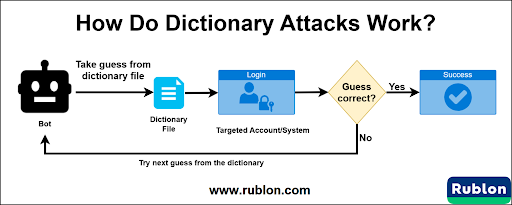
\includegraphics[scale=0.6]{pic/dictionary.png}
    \caption{Cách cuộc tấn công Dictionary hoạt động}
\end{figure}
Loại tấn công này sử dụng một phương pháp hệ thống để phá vỡ mật khẩu. Có ba bước cơ bản để thực hiện những cuộc tấn công này một cách thành công và hiểu rõ chúng có thể hữu ích trong việc học cách ngăn chặn một cuộc tấn công từ điển.\\

Thường thì, kẻ tấn công sẽ tạo ra một danh sách trước định các mật khẩu tiềm năng - một từ điển tấn công thô mà bao gồm các kết hợp của các từ phổ biến và số.
Phần mềm tự động sau đó sử dụng từ điển tấn công này để thử tấn công vào các tài khoản trực tuyến.\cite{bovsnjak2018brute}
Sau khi cuộc tấn công từ điển đã thành công tấn công vào một tài khoản dễ bị tấn công, kẻ tấn công sử dụng bất kỳ dữ liệu nhạy cảm nào được lưu trữ trong hồ sơ cho mục đích của riêng họ. Điều này có thể là để gian lận, thực hiện hành động độc hại, hoặc đơn giản là truy cập vào các tài khoản với mục đích tài chính.\\

Để biên soạn danh sách các mật khẩu tiềm năng, kẻ tấn công thường sử dụng tên thú nuôi phổ biến, nhân vật văn hóa đại chúng nhận dạng hoặc các đội thể thao và vận động viên nổi tiếng, ví dụ. Điều này là do nhiều người sử dụng loại từ này để tạo ra các mật khẩu có ý nghĩa với họ và mà họ có thể nhớ dễ dàng. Danh sách thường sẽ bao gồm các biến thể của chúng, như các kết hợp từ khác nhau, hoặc sự thêm vào của các ký tự đặc biệt.\\

Chạy danh sách này với các công cụ tự động cũng làm cho cuộc tấn công từ điển trở nên dễ dàng thành công hơn. Sử dụng danh sách mật khẩu và công cụ tự động cùng nhau khiến việc cố gắng phá vỡ mật khẩu và tấn công vào một tài khoản trực tuyến nhanh chóng hơn đáng kể. Nếu việc này được thực hiện thủ công thì cuộc tấn công sẽ mất quá nhiều thời gian và cho phép chủ sở hữu tài khoản hoặc quản trị hệ thống phát hiện và triển khai một phòng thủ chống lại cuộc tấn công.\\

Bởi vì cách chúng hoạt động, những cuộc tấn công từ điển thường không có một mục tiêu cá nhân. Thay vào đó, chúng được thực hiện với hi vọng một trong số các mật khẩu trên danh sách sẽ chính xác. Tuy nhiên, nếu kẻ tấn công đang nhắm vào một địa điểm hoặc tổ chức cụ thể, họ sẽ tạo ra một danh sách từ cụ thể và cục bộ hơn. Ví dụ, nếu họ có kế hoạch thực hiện cuộc tấn công ở Tây Ban Nha, họ có thể sử dụng các từ Tây Ban Nha phổ biến thay vì tiếng Anh. Hoặc, nếu họ đang nhắm vào một tổ chức cụ thể, họ có thể sử dụng các từ liên quan đến công ty đó.
\subsubsection{Nguyên nhân người dùng bị tấn công Dictionary}

\begin{itemize}
    \item \textbf{Sử dụng mật khẩu yếu}: Nhiều người dùng sử dụng các mật khẩu đơn giản, dễ đoán như "123456", "password", hay "abc123". Những mật khẩu này thường nằm trong danh sách từ điển mật khẩu của kẻ tấn công.
    \item \textbf{Mật khẩu phổ biến}: Có những mật khẩu phổ biến mà nhiều người dùng chọn vì dễ nhớ. Kẻ tấn công sẽ thử những mật khẩu này trước vì khả năng thành công cao hơn.
    \item \textbf{Không thay đổi mật khẩu thường xuyên}: Khi người dùng không thay đổi mật khẩu định kỳ, khả năng mật khẩu bị lộ và nằm trong danh sách từ điển của kẻ tấn công tăng lên.
    \item \textbf{Tái sử dụng mật khẩu}: Nhiều người dùng sử dụng cùng một mật khẩu cho nhiều tài khoản khác nhau. Nếu một tài khoản bị lộ, các tài khoản khác cũng có nguy cơ bị tấn công.
    \item \textbf{Thiếu ký tự đặc biệt và độ dài mật khẩu}: Mật khẩu ngắn và thiếu ký tự đặc biệt (chữ hoa, chữ thường, số, ký tự đặc biệt) dễ bị bẻ khóa hơn vì có ít sự kết hợp để thử.
    \item \textbf{Thông tin cá nhân trong mật khẩu}: Sử dụng thông tin cá nhân như tên, ngày sinh, hoặc số điện thoại làm mật khẩu khiến mật khẩu dễ bị đoán ra.
    \item \textbf{Không sử dụng xác thực hai yếu tố (2FA)}: Thiếu các biện pháp bảo vệ bổ sung như xác thực hai yếu tố làm cho việc bẻ khóa mật khẩu dễ dàng hơn.
\end{itemize}
\subsubsection{ Các công cụ dùng trong tấn công}
\begin{itemize}
    \item \textbf{John the Ripper}: Đây là một trong những công cụ bẻ khóa mật khẩu phổ biến nhất. Nó hỗ trợ nhiều định dạng mật khẩu và có thể sử dụng các tập tin từ điển để thử các mật khẩu phổ biến.
    \item \textbf{Hashcat}: Đây là một công cụ mạnh mẽ hỗ trợ bẻ khóa mật khẩu sử dụng GPU, giúp tăng tốc độ tấn công. Hashcat có thể thực hiện nhiều loại tấn công, bao gồm tấn công từ điển.
    \item \textbf{Aircrack-ng}: Bộ công cụ này thường được sử dụng để kiểm tra bảo mật mạng Wi-Fi. Nó có thể thực hiện tấn công từ điển để bẻ khóa mật khẩu WPA và WPA2.
    \item \textbf{Hydra}: Đây là một công cụ rất mạnh mẽ cho các tấn công Brute Force và từ điển trên các giao thức mạng. Nó hỗ trợ nhiều giao thức như FTP, HTTP, SMB, và nhiều hơn nữa.
    \item \textbf{Cain \& Abel}: Đây là một công cụ phục hồi mật khẩu dành cho Windows, hỗ trợ nhiều kỹ thuật bẻ khóa mật khẩu khác nhau, bao gồm tấn công từ điển.
    \item \textbf{Medusa}: Một công cụ tấn công mật khẩu dựa trên từ điển và Brute Force. Medusa được thiết kế để kiểm tra bảo mật mật khẩu trên nhiều giao thức.
    \item \textbf{THC Hydra}: Đây là một công cụ mạng mạnh mẽ để thực hiện tấn công mật khẩu từ điển. Hydra có khả năng tấn công nhiều giao thức khác nhau, từ SSH đến Telnet.
    \item \textbf{Ophcrack}: Một công cụ chuyên dụng cho việc bẻ khóa mật khẩu Windows sử dụng các bảng rainbow (rainbow tables), nhưng cũng có thể sử dụng từ điển mật khẩu để thực hiện tấn công từ điển.
    \item \textbf{Patator}: Đây là một công cụ tấn công mật khẩu đa năng, hỗ trợ nhiều loại tấn công khác nhau, bao gồm tấn công từ điển trên các dịch vụ như SSH, FTP, HTTP, và nhiều hơn nữa.
\end{itemize}